%================文档声明==================
% a4纸张大小，基本字号为12pt(小四),编码为UTF8,
\documentclass[a4paper,12pt,UTF8,hyperref]{ctexart} 

%==========================使用彩色=============================
%\usepackage[usenames,dvipsnames]{color}
\usepackage{color}
\usepackage[table]{xcolor}
\usepackage{colortbl}
\definecolor{mygray}{gray}{.9}
\definecolor{mypink}{rgb}{.99,.91,.95}
\definecolor{mycyan}{cmyk}{.3,0,0,0}
\definecolor{darkred}{HTML}{8B0000}  % 深红色，用于交叉引用等内部链接
%================================================================

%========================电子文档与超链接======================
\usepackage[backref=page,hyperfootnotes=false]{hyperref}
\hypersetup{
 %bookmarks = true,   % 启用pdf书签
 bookmarksopen = true,   % 打开pdf时，书签默认展开
 pdfborder=0 0 0,      % 控制pdf超链接的边框
 %hyperfootnotes=false,   % 页脚不会跳转
 pdfpagemode = FullScreen,   % 打开pdf时全屏模式
 pdfstartview = Fit,  % 打开时主动适应窗口
 pdftitle = {本科毕业设计(论文)},  % pdf文件的属性
 colorlinks = true,   % 链接用文字颜色标识，不画边框
 linkcolor = darkred,   % 交叉引用（\ref、\cref、图表、公式等）为深红色
 citecolor = darkred,   % 文献引用为深红色
 urlcolor = darkred,   % 网址/DOI 为深红色
 linktoc = all,   % 目录中的标题和页码都可点击
}
\pdfbookmark[1]{Contents}{contents}
%===============================================================

%=======================字体与基本格式===========================
\usepackage{fontspec}  % 提供系统字体调节能力
\usepackage{xeCJK}  % 提供中文支持
\usepackage[a4paper,left=3.0cm,right=2.0cm,top=2.5cm,bottom=3cm]{geometry}   % 整体页面大小设置
\setmainfont{Times New Roman}%全文英文字体使用Times New Roman；
\linespread{1.5}%全文1.5倍行距；
\setCJKfamilyfont{hwxw}{STXinwei}      % 定义华文新魏  h
\newcommand{\hwxw}{\CJKfamily{hwxw}}
%=============================================================

%========================设置页眉以及页脚基本格式===========================
\usepackage{fancyhdr}% 为了保证正确长度的页眉下划线,fancyhdr宏包要在geometry宏包后使用；
\usepackage{lastpage}  % 获取总页数，正文要用
\pagestyle{fancy}
\fancyhf{}  % 清空原有页眉页脚
\setlength{\headheight}{27pt}   % 设置页眉大小
\setlength{\headsep}{1em}  % 页眉底部到正文顶部距离
\fancyhead[L]{
\includegraphics[scale=0.125]{./figures/CSU_Logo.jpg}}
\fancyhead[R]{\small\heiti 基于多模型融合的红茶发酵程度识别算法研究}
\setlength{\footskip}{2em}
% 页脚具体样式在document中设置，以满足不同页的不同要求
%===============================================================

%==========================目录格式===============================
\usepackage{titletoc}  % 定制目录样式

% section在目录中的样式
\titlecontents{section}
  [0em]                                  % 左缩进
  {\normalsize}                           % 字体
  {第\makebox[1em][c]{\thecontentslabel}章\quad}       % ★ 编号格式
  {}                                     % 无编号时,及结束语、参考文献、附录
  {\titlerule*[4pt]{.}\contentspage}     % 点线+页码
  
\titlecontents{subsection}
  [2em]                                  % 左缩进
  {\normalsize}                           % 字体
  {\makebox[1em][c]{\thecontentslabel}\quad}       % ★ 编号格式
  {}                                     % 无编号时,及结束语、参考文献、附录
  {\titlerule*[4pt]{.}\contentspage}     % 点线+页码

\titlecontents{subsubsection}
  [4em]                                  % 左缩进
  {\normalsize}                           % 字体
  {\thecontentslabel\quad}       % ★ 编号格式
  {}                                     % 无编号时,及结束语、参考文献、附录
  {\titlerule*[4pt]{.}\contentspage}     % 点线+页码
%===============================================================


%========================章节及子标题格式=============================
\usepackage{titlesec}  % 自定义章节格式
\usepackage{indentfirst} % 每章第一正文也缩进
\setlength{\parindent}{2em} % 缩进宽度为2em

% 一二三级标题格式
\titleformat{\section}[hang]{\heiti\zihao{3}\center}{第\makebox[1em][c]{\thesection}章 \quad}{0pt}{}{}  %一级标题格式
\titleformat{\subsection}[hang]{\heiti\zihao{-4}}{\thesubsection \quad}{0pt}{}{} % 二级标题格式
\titleformat{\subsubsection}[hang]{\zihao{-4}\kaishu}{\thesubsubsection \quad}{0pt}{}{} %三级标题格式

% 设置标题边距，顺序为左上下正文
\titlespacing*{\section}{2em}{1em}{1em}[0pt]  
\titlespacing*{\subsection}{2em}{0pt}{0pt}[0pt]
\titlespacing*{\subsubsection}{2em}{0pt}{0pt}[0pt]
%===============================================================

%==========================插入图片===================================
\usepackage{graphicx}
\usepackage{picinpar}%文字绕排
\usepackage{caption}
\usepackage{subcaption}  %两图并排
\captionsetup{font=small,labelfont=bf,labelsep=quad}
\captionsetup{skip=0pt}%标题与浮动环境内容的垂直间距无额外间距（设置为0pt）;
%====================================================================

%===============================插入表格======================================
\usepackage{booktabs,multirow}%三线表
\usepackage{longtable}%长表格
\usepackage{bigstrut}
\usepackage{diagbox}
\usepackage{makecell}
\usepackage{tabularx}
\newcolumntype{Y}{>{\centering\arraybackslash}X}  % 新定义列形式，表格自动填满空行，并保持字体居中
%=============================================================================

%==========================解决三线表竖线过短的问题=============================
\renewcommand{\cmidrulesep}{0mm} %定义两条相邻\cmidrule之间的间隔
\setlength{\aboverulesep}{0mm} %在线条[不包括\toprule]上面增加一段垂直距离，此处为0mm
\setlength{\belowrulesep}{0mm} %在线条[不包括\bottomrule]下面增加一条垂直距离，此处为0mm
\setlength{\abovetopsep}{0cm}  %在线条\toprule上面，即表格与上面的文字之间的距离。
\setlength{\belowbottomsep}{0cm}%在线条\bottomrule下面，即表格与下面的文字之间的距离。
%===============================================================

%==========================数学公式=============================
\usepackage{amsmath}%公式
\usepackage{amssymb}
\usepackage{bm}%粗体
\usepackage{upgreek}%直立希腊字母
\usepackage{mhchem}%化学公式 \ce{SiO2} 或 \ce{H2O}
\DeclareMathOperator\dif{d\!}%微分算子\frac{\dif y}{dif x}
%\usepackage{xfrac}%行内小分式
\newenvironment{sequation}{\begin{equation}\small}{\end{equation}}
\newenvironment{tequation}{\begin{equation}\tiny}{\end{equation}}
%===============================================================

%=======================附录格式所需宏包=========================
\usepackage{cleveref}  % cleveref的插入必须在amsmat之后，并且正文中可以直接使用/cref
%=============================================================

%==========================程序代码=============================
\usepackage{listings}
\usepackage{pythonhighlight}
%===============================================================

%=============================其它===============================
\usepackage{siunitx}%摄氏度 \SI{100}{\degreeCelsius}
\makeatletter%罗马数字
\newcommand{\rmnum}[1]{\romannumeral #1}% 罗马数字
\newcommand{\Rmnum}[1]{\expandafter\@slowromancap\romannumeral #1@}%罗马数字
\makeatother%罗马数字 \Rmnum{1} 或 \Rmnum{2} 或 \rmnum{3}
\usepackage{xfrac}%行内小分式
%==================================================================

%=============================文献格式===============================
\usepackage[sort]{gbt7714}%文献格式使用GB/T7714-2015标准；
\newcommand{\upcite}[1]{\textsuperscript{\textsuperscript{\cite{#1}}}}
\usepackage{natbib}
\renewcommand\bibfont{\small\kaishu}%文献改用5号楷书字体；
\setlength\bibsep{0pt}%取消不同文献条目之间的距离；
\usepackage{url}
%==================================================================

%=========================一个更好的下划线设置=======================
\usepackage{ulem}
\usepackage{enumitem}
\usepackage{hhline}% 双线表
\newcommand\dlmu[2][4cm]{\hskip1pt\underline{\hb@xt@ #1{\hss#2\hss}}\hskip3pt}
%==================================================================

%=========================公式、图表按章编号===============================
\makeatletter
\@addtoreset{equation}{section}
\makeatother
\renewcommand{\theequation}{\arabic{section}-\arabic{equation}}

\makeatletter
\@addtoreset{figure}{section}
\makeatother
\renewcommand{\thefigure}{\thesection\,-\,\arabic{figure}}

\makeatletter
\@addtoreset{table}{section}
\makeatother
\renewcommand{\thetable}{\thesection\,-\,\arabic{table}}
%==================================================================

\usepackage{ifpdf}

\newtheorem{thm}{定理}

%==============积分符号修改，改原倾斜的积分符号为直立体==================
\usepackage{amsmath,amssymb}
\DeclareSymbolFont{EulerExtension}{U}{euex}{m}{n}
\DeclareMathSymbol{\euintop}{\mathop} {EulerExtension}{"52}
\DeclareMathSymbol{\euointop}{\mathop} {EulerExtension}{"48}
\let\intop\euintop
\let\ointop\euointop
%==================================================================

%=====================图标引用格式的修改=========================
% 表格
\crefname{table}{表}{表}
\Crefname{table}{表}{表}
\creflabelformat{table}{#2~#1#3}  

% 子表
\crefname{subtable}{表}{表}
\Crefname{subtable}{表}{表}
\creflabelformat{subtable}{#2~#1#3}

% 图
\crefname{figure}{图}{图}
\Crefname{figure}{图}{图}
\creflabelformat{figure}{#2~#1#3}

% 子图
\crefname{subfigure}{图}{图}
\Crefname{subfigure}{图}{图}
\creflabelformat{subfigure}{#2~#1#3}
%================================================================


% =========================== 以下是文章表示==============================
\usepackage{doc}%BibTeX显示；
\begin{document}
    % 封面页
    % ====这里是首页的格式定义
\begin{titlepage}
  % 中南大学logo
  \begin{figure}[htbp]
    \centering
    
\includegraphics[scale=0.58]{./figures/CSU_Logo.jpg}\\
  \end{figure}

  \phantom{ 空一行，不显示}

  % 封面标题，45磅黑体字，居中
  \begin{center}
      {\fontsize{45pt}{55pt}\heiti{本科毕业论文（设计）}}
  \end{center}

  \phantom{ 空小行，不显示}
  % 封面英文标题
  \begin{center}
      {\zihao{1}\heiti GRADUATION THESIE(DESIGN)}
  \end{center}

  \phantom{ 空两行：1}


  \begin{table}[htbp]
    \centering\zihao{-2}\kaishu
    
      \begin{tabular}{c >{\centering\arraybackslash}m{7.4cm}}
        {\heiti 题\qquad 目： }& 基于多模型融合的红茶发酵程度识别算法研究 \\
            \cline{2-2}  % 下划横线
        {\heiti 学\qquad 生：}&  NONG \\
            \cline{2-2}
        {\heiti 学\qquad 号：}&  20260120\\
          \cline{2-2}
        {\heiti 专业班级：}& 计算机科学与技术2206班\\
          \cline{2-2}
        {\heiti 指导教师：}& 大佬 \\
            \cline{2-2}
        {\heiti 学\qquad 院：}&  计算机学院 \\
            \cline{2-2}
      \end{tabular}
  \end{table}

  \vspace{2em}

  \begin{center}
    \zihao{2}{\heiti 本科生院制}\\
    \zihao{-2}{\heiti 2026年5月}
  \end{center}

\end{titlepage}

  
    \clearpage 

    % 学位论文原创性声明-2026新增
    \thispagestyle{empty}  % 本页不显示页眉页脚
\phantom{空一行}
\begin{center}
    {\hwxw \zihao{2} 学位论文原创性声明}
\end{center}

    本人郑重声明，所呈交的学位论文是本人在导师指导下进行的研究工作及取得的研究成果。
尽我所知，除了论文中特别加以标注和致谢的地方外，论文中不包含其他人已经发表或撰写过的研究成果，
也不包含为获得中南大学或其他教育机构的学位或证书而使用过的材料。与我共同工作的同志对本研究所作的贡献均已在论文中作了明确的说明。

    申请学位论文与资料若有不实之处，本人承担一切相关责任。

\vspace{1em}

    学位论文作者签名：\underline{\hspace{7em}}\hspace{2em}日期：\underline{\hspace{4.5em}}年\underline{\hspace{2.5em}}月\underline{\hspace{2.5em}}日

\vspace{3em}
\begin{center}
    {\hwxw \zihao{2} 学位论文版权使用授权书}
\end{center}

    本学位论文作者和指导教师完全了解中南大学有关保留、使用学位论文的规定：即学校有权保留并向国家有关部门或机构送交学位论文的复印件和电子版，
允许本学位论文被查阅和借阅。本人授权中南大学可以将本学位论文的全部或部分内容编入有关数据库进行检索和公开传播，可以采用复印、缩印或其它手段保存和汇编学位论文。
本人保证：毕业后以学位论文内容发表的论文作者单位注明中南大学；学位论文电子文档的内容和纸质学位论文的内容相一致。

    延缓公开论文延缓到期后适用本授权书，涉密论文在解密后适用本授权书。

\vspace{1em}

    本学位论文属于：(请在以下相应方框内打“$\checkmark$”）

    $\square$公开

    $\square$延缓公开，延缓期限（\underline{\hspace{3.5em}}年\underline{\hspace{2em}}月\underline{\hspace{2em}}日
    至\underline{\hspace{3.5em}}年\underline{\hspace{2em}}月\underline{\hspace{2em}}日）


\vspace{2em}

\noindent
\begin{tabular}{l l}
学位论文作者签名：   \underline{\hspace{7em}   }      &       \hspace{2em}指导教师签名 ： \underline{\hspace{9em} }     \\  
日期：\underline{\hspace{4.5em}}年\underline{\hspace{2.5em}}月\underline{\hspace{2.5em}}日  &     \hspace{2em}日期：\underline{\hspace{4.5em}}年\underline{\hspace{2.5em}}月\underline{\hspace{2.5em}}日 \\
（填写阿拉伯数字）

\end{tabular}




    \clearpage

    % 摘要页及目录页 
    % 1.页脚格式：罗马大写字母
    \setcounter{page}{1}
    \pagenumbering{Roman}
    \cfoot{\small\thepage}

    % 2.引入摘要页
    \phantom{空一行}
\vspace{-2em} % 修正
\begin{center}
	\zihao{-2}\heiti
	基于多模型融合的红茶发酵程度识别算法研究
\end{center}

\begin{center}
	\zihao{3}\heiti
	\phantomsection   % 锚点，编译后的pdf可以直接跳转
	摘要
\end{center}

\vspace{0.5em} % center自带一定空行

这里是摘要，请好好写。本文的参考文献用于举例参考文献引用方法\cite{DP图像分类综述}。本文的附录用于举例附录引用方法如“见附录\ref{matlab_example}和附录\ref{python_example}”。

\vspace{1em}  

\noindent
\textbf{关键字：}关键字1\quad 关键字2\quad 关键字3
\newpage

\phantom{空一行}
\vspace{-2em} % 向上修正页眉与正文之间的统一空行1em
\begin{center}
	\zihao{-2}\bfseries
	\rmfamily Research on a Multi‑Model Fusion Algorithm for Black Tea Fermentation Degree Recognition
\end{center}

\begin{center}
	\phantomsection
	\zihao{3}\rmfamily\bfseries
	ABSTRACT
\end{center}

\vspace{0.5em}  % center自带一定空行

This is abstract. Literature are for example\cite{DP图像分类综述}.The appendix of this article is used for example, like this "See Appendix \ref{matlab_example} for details".

\vspace{1em}

\noindent\textbf{Key Words:}\quad Key1\quad Key2\quad Key3\quad Key4

    \newpage

    % 目录页
    \phantom{空一行}
    \vspace{-1em} % 向上修正页眉与正文之间的统一空行1em
    % 目录文字（含页码）设为黑色：仅在目录范围内把链接颜色改为黑色，
    % 目录之后恢复 \hypersetup 中的深红色，不影响正文交叉引用
    \begingroup
    \hypersetup{linkcolor=black}
    \tableofcontents
    \endgroup
    \newpage

    % 正文
    \setcounter{page}{1}
    \pagenumbering{arabic}
    \cfoot{\small 第\ \thepage\ 页\quad 共 \pageref{LastPage} 页}
    
\section{图}
	Python代码示例见附录\ref{python_example}，作为附录引用示例。这里是第一个脚注\footnote{第一个脚注示例}，这里是第二个脚注\footnote{第二个脚注示例}
	\subsection{单图示例}
		这是一个单图示例，这个单图的详情见\cref{fig:单图}
		\begin{figure}[htbp]
			\centering
			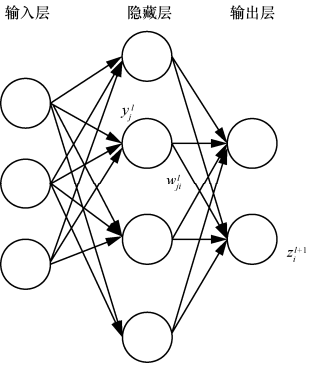
\includegraphics[width = 0.3\textwidth]{./figures/神经网络前向传播.png}
			\caption{这个是单图}
			\label{fig:单图}
		\end{figure}

		上面写了一个单图，接下来写双图

	\subsection{双图示例}

		\subsubsection{两个并列的图}
			\begin{figure}[htbp]
				\centering
				\begin{subfigure}{0.45\textwidth}
					\centering
					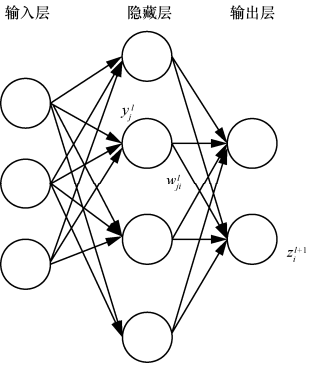
\includegraphics[width = 0.7\textwidth]{./figures/神经网络前向传播.png}
					\caption{这个是双图1}
					\label{fig:双图1}
				\end{subfigure}
				\begin{subfigure}{0.45\textwidth}
					\centering
					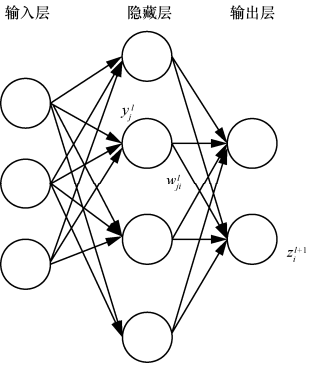
\includegraphics[width = 0.7\textwidth]{./figures/神经网络前向传播.png}
					\caption{这个是双图2}
					\label{fig:双图2}
				\end{subfigure}
				\caption{这里是双图}
			\end{figure}

		双图的引用，可见第一张图：\cref{fig:双图1}，以及第二张图：\cref{fig:双图2}

		\subsubsection{一个图，但是左边有说明}
			\begin{figure}[htbp]
				\centering
				\begin{minipage}[c]{0.45\textwidth}
					\centering
					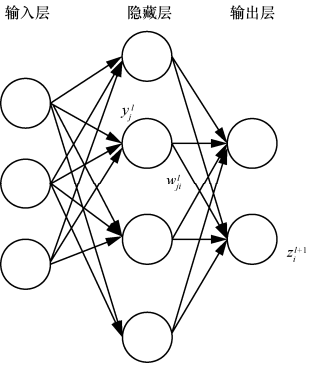
\includegraphics[width=0.7\textwidth]{./figures/神经网络前向传播.png}
					\caption{这是一个有说明的单图}
					\label{fig:说明单图}
				\end{minipage}
				\begin{minipage}[l]{0.45\textwidth}
					 这里是图像说明：这是个神经网络，它有如下特点:

					\begin{itemize}
						\item 有输入层
						\item 有隐藏层
						\item 有输出层
					\end{itemize}

				\end{minipage}
			\end{figure}
		
\newpage


\section{表}
	\subsection{单三线表的示例}
		\begin{table}[htbp]
			\centering
			\caption{不同模型在测试集上的准确率（瞎编版）}
			\label{tab:不同模型的测试结果}
			\begin{tabularx}{\textwidth}{YYYY}
				\toprule
				模型 			& Precision 		& Recall 			& Accuracy \\
				\midrule
				ResNet101 		& 0.91 				& 0.89 				& 0.90 \\
				VGG16     		& 0.88 				& 0.86 				& 0.87 \\
				ViT       		& 0.93 				& 0.92 				& 0.92 \\
				EfficientNet	& 0.92 				& 0.91 				& 0.91 \\
				\textbf{ours}   & \textbf{0.96} 	& \textbf{0.93} 	& \textbf{0.94} \\
				\bottomrule
			\end{tabularx}
		\end{table}

		上面做了三线表的示例，见\cref{tab:不同模型的测试结果}，接下来试试并列双三线表。

	\subsection{双三线表的示例}
		\begin{table}[htbp]
			\centering
			\caption{实验结果（瞎编版）}
			\label{tab:双表示例}
			
			\begin{subtable}[t]{0.45\textwidth}
				\centering
				\caption{消融实验：数据预处理}
				\label{tab:消融实验：数据预处理}
				\begin{tabularx}{0.95\textwidth}{YYY}
					\toprule
					模型 			& Pre Acc  		 	            & Acc \\
					\midrule
					ResNet101 		& 0.90 							& 0.92 \\
					VGG16     		& 0.88 			 				& 0.95 \\
					ViT       		& 0.93 			 				& 0.92 \\
					EfficientNet	& 0.92 			 				& 0.95 \\
					\textbf{ours}   & \textbf{0.93} 			 	& \textbf{0.97} \\
					\bottomrule
				\end{tabularx}
			\end{subtable}
			\hfill   % 注意这里hfill上下不能空行，才能强行将两个表拉成水平
			\begin{subtable}[t]{0.45\textwidth}
				\centering
				\caption{消融实验：数据增强}
				\label{tab:消融实验：数据增强}
				\begin{tabularx}{0.95\textwidth}{YYY}
					\toprule
					模型 			& Pre Acc  		 	            & Acc \\
					\midrule
					ResNet101 		& 0.90 							& 0.92 \\
					VGG16     		& 0.88 			 				& 0.95 \\
					ViT       		& 0.93 			 				& 0.92 \\
					EfficientNet	& 0.92 			 				& 0.95 \\
					\textbf{ours}   & \textbf{0.93} 			 	& \textbf{0.97} \\
					\bottomrule
				\end{tabularx}
			\end{subtable}
		\end{table}

		并列双三线表的示例见\cref{tab:双表示例} ，两个子表分别见\cref{tab:消融实验：数据增强}，以及\cref{tab:消融实验：数据预处理}。

	\subsection{跨页三线表的示例}
		当表格超出一页时，三线表需要用 \texttt{longtable} 环境排版。跨页三线表有两个要求：一是\textbf{表头在每一页重复}，二是\textbf{续页表头要写“表-x 续”，并保留表题说明}，使读者只看续页也能知道该表的内容。跨页三线表的示例如\cref{tab:跨页三线表}。

		\newpage

		\begin{longtable}{@{}c>{\centering\arraybackslash}p{0.26\textwidth}*{4}{>{\centering\arraybackslash}p{0.13\textwidth}}@{}}
			%========== 第一页：表题 + 表头 ==========
			\caption{不同模型在各轮实验中的性能对比（瞎编版，用于演示跨页）}
			\label{tab:跨页三线表}\\
			\toprule
			序号 & 模型 & 参数量/M & Precision & Recall & Accuracy \\
			\midrule
			\endfirsthead

			%========== 续页：重复表头，表题标注“表-x 续”并保留表题说明 ==========
			\multicolumn{6}{c}{\small 表\thetable\ 续\quad 不同模型在各轮实验中的性能对比}\\
			\toprule
			序号 & 模型 & 参数量/M & Precision & Recall & Accuracy \\
			\midrule
			\endhead

			%========== 除末页外，每页底部画线 ==========
			\bottomrule
			\endfoot

			%========== 末页底部画线 ==========
			\bottomrule
			\endlastfoot

			1  & ResNet18        & 11.7   & 0.81 & 0.79 & 0.80 \\
			2  & ResNet50        & 25.6   & 0.84 & 0.83 & 0.83 \\
			3  & ResNet101       & 44.5   & 0.87 & 0.85 & 0.86 \\
			4  & VGG16           & 138.4  & 0.83 & 0.81 & 0.82 \\
			5  & ViT-B/16        & 86.6   & 0.89 & 0.88 & 0.88 \\
			6  & Swin-T          & 28.3   & 0.90 & 0.89 & 0.89 \\
			7  & EfficientNet-B0 & 5.3    & 0.87 & 0.85 & 0.86 \\
			8  & MobileNetV3     & 5.4    & 0.85 & 0.83 & 0.84 \\
			9  & ResNet18        & 11.7   & 0.82 & 0.80 & 0.81 \\
			10 & ResNet50        & 25.6   & 0.85 & 0.84 & 0.84 \\
			11 & ResNet101       & 44.5   & 0.88 & 0.86 & 0.87 \\
			12 & VGG16           & 138.4  & 0.84 & 0.82 & 0.83 \\
			13 & ViT-B/16        & 86.6   & 0.90 & 0.89 & 0.89 \\
			14 & Swin-T          & 28.3   & 0.91 & 0.90 & 0.90 \\
			15 & EfficientNet-B0 & 5.3    & 0.88 & 0.86 & 0.87 \\
			16 & MobileNetV3     & 5.4    & 0.86 & 0.84 & 0.85 \\
			17 & ResNet18        & 11.7   & 0.83 & 0.81 & 0.82 \\
			18 & ResNet50        & 25.6   & 0.86 & 0.85 & 0.85 \\
			19 & ResNet101       & 44.5   & 0.89 & 0.87 & 0.88 \\
			20 & VGG16           & 138.4  & 0.85 & 0.83 & 0.84 \\
			21 & ViT-B/16        & 86.6   & 0.91 & 0.90 & 0.90 \\
			22 & Swin-T          & 28.3   & 0.92 & 0.91 & 0.91 \\
			23 & EfficientNet-B0 & 5.3    & 0.89 & 0.87 & 0.88 \\
			24 & MobileNetV3     & 5.4    & 0.87 & 0.85 & 0.86 \\
			25 & ResNet18        & 11.7   & 0.84 & 0.82 & 0.83 \\
			26 & ResNet50        & 25.6   & 0.87 & 0.86 & 0.86 \\
			27 & ResNet101       & 44.5   & 0.90 & 0.88 & 0.89 \\
			28 & VGG16           & 138.4  & 0.86 & 0.84 & 0.85 \\
			29 & ViT-B/16        & 86.6   & 0.92 & 0.91 & 0.91 \\
			30 & Swin-T          & 28.3   & 0.93 & 0.92 & 0.92 \\
			31 & EfficientNet-B0 & 5.3    & 0.90 & 0.88 & 0.89 \\
			32 & MobileNetV3     & 5.4    & 0.88 & 0.86 & 0.87 \\
			33 & ResNet18        & 11.7   & 0.85 & 0.83 & 0.84 \\
			34 & ResNet50        & 25.6   & 0.88 & 0.87 & 0.87 \\
			35 & ResNet101       & 44.5   & 0.91 & 0.89 & 0.90 \\
			36 & VGG16           & 138.4  & 0.87 & 0.85 & 0.86 \\
			37 & ViT-B/16        & 86.6   & 0.93 & 0.92 & 0.92 \\
			38 & Swin-T          & 28.3   & 0.94 & 0.93 & 0.93 \\
			39 & EfficientNet-B0 & 5.3    & 0.91 & 0.90 & 0.90 \\
			40 & MobileNetV3     & 5.4    & 0.89 & 0.87 & 0.88 \\
			41 & ResNet18        & 11.7   & 0.86 & 0.84 & 0.85 \\
			42 & ResNet50        & 25.6   & 0.89 & 0.88 & 0.88 \\
			43 & ResNet101       & 44.5   & 0.92 & 0.90 & 0.91 \\
			44 & VGG16           & 138.4  & 0.88 & 0.86 & 0.87 \\
			45 & ViT-B/16        & 86.6   & 0.94 & 0.93 & 0.93 \\
			46 & Swin-T          & 28.3   & 0.95 & 0.94 & 0.94 \\
			47 & EfficientNet-B0 & 5.3    & 0.92 & 0.91 & 0.91 \\
			48 & \textbf{Ours}   & \textbf{23.1} & \textbf{0.97} & \textbf{0.95} & \textbf{0.96} \\
		\end{longtable}

		跨页三线表见\cref{tab:跨页三线表}：第一页显示完整表题，表格跨页后，续页顶部会重复表头，并把表题写成“表\ref{tab:跨页三线表} 续\quad 不同模型在各轮实验中的性能对比”的形式（编号自动跟随当前表格，表题说明建议与首页保持一致）。
\newpage

\section{公式}
	\subsection{对齐的长等式}
		
		\begin{align}
			\label{alg:交叉熵损失 }
			\mathcal{L}(\theta)
								&= - \sum_{i=1}^{N} \log p_\theta(y_i \mid x_i)  \nonumber\\
								&= - \sum_{i=1}^{N} \log   \frac{\exp(f_\theta(x_i, y_i))}
											{\sum_{k=1}^{K} \exp(f_\theta(x_i, k))}  \nonumber  \\
								&= - \sum_{i=1}^{N} f_\theta(x_i, y_i)
											+ \sum_{i=1}^{N} \log \sum_{k=1}^{K}
											\exp(f_\theta(x_i, k)) \ .
		\end{align}

	公式示例如\cref{alg:交叉熵损失 }

\newpage

\phantom{ 空一行}
\vspace{-2em}  %修正
\begin{center}
	\zihao{3}\heiti
	\phantomsection
	\addcontentsline{toc}{section}{结\hspace{0.5em}束\hspace{0.5em}语}
	结束语
\end{center}

这里结束语/致谢。可以顺便致谢一下这个模板（doge）。喜欢的学弟学妹别忘了
点个star :)
    \newpage

    % 参考文献  
    \addcontentsline{toc}{section}{参考文献}
    \nocite{*}  % 不论有没有引用，都放在文献列表中
    \bibliographystyle{gbt7714-numerical}%命令选择参考文献样式 
    \bibliography{./literature/thesis}    % 引入参考文件bib
    \newpage

    % 附录
    % 以section形式将附录加入到目录中
\addcontentsline{toc}{section}{附\hspace{2em}录}
\phantomsection    % 创建目录超链接目标
\phantom{ 空一行 }
\vspace{-1em}    % 修正center自带空行
\begin{center}
	{\zihao{3}\heiti 附\qquad 录}
\end{center}

% 代码格式的设置
\lstset{
  basicstyle=\ttfamily\small,  % 设置基本字体
  frame= shadowbox,   % 添加带阴影的边框
  numbers=left,     % 行号显示在左侧
  numberstyle=\tiny\color{gray},  % 行号颜色为灰色，tiny字体
  keywordstyle=\color{blue},    % 关键字 for ,while ,if等，改为蓝色
  commentstyle=\color{green},   % 注释样式：绿色
  stringstyle=\color{red},   % 字符串显示样式：红色
  breaklines=true,     % 长代码自动换行
  showstringspaces=true  % 字符串中的空格不显示
}

\newcounter{appendix_counter}
\newcommand{\theappsub}{\arabic{appendix_counter}}  % 新定义编号引用命令
\crefname{appsub}{附录}{附录}    % 定义正文进行\ref时所使用的格式


% 以subsection形式加入到目录当中
\refstepcounter{appendix_counter}   % 建立/ref节点 , counter会自动+1
\addcontentsline{toc}{subsection}{\theappsub \hspace{1em} Matlab代码示例 }  % 添加到目录中
\phantomsection
\arabic{appendix_counter}\hspace{1em} {\heiti\zihao{-4} Matlab代码示例}  % 标题
	\lstinputlisting[language=Matlab, label={matlab_example}]
		{codes/matlabcode.m}
\vspace{1em}

\refstepcounter{appendix_counter} 
\addcontentsline{toc}{subsection}{\theappsub\hspace{1em} Python代码示例 } 
\phantomsection
\arabic{appendix_counter}\hspace{1em} {\heiti\zihao{-4} Python代码示例}
	\lstinputlisting[language=Python, label={python_example}]
		{codes/pythoncode.py}

\end{document}
